% !TEX root = pfc.tex

O tráfego de veículos representa um fenômeno de grande importância socioeconômica, principalmente nos grandes centros urbanos cujos deslocamentos, no menor tempo possível, são uma necessidade cotidiana. Projetar sistemas viários que absorvam toda a frota veicular desses grandes centros e minimizam os congestionamentos exige ferramentas cujo desenvolvimento ainda representa objeto de estudo para diversos grupos de pesquisadores.

Vários fatores interferem na qualidade do tráfego, sendo o principal o crescente número de veículos nos centros urbanos. Segundo \cite{fenabrave:2013:online} - Federação Nacional da Distribuição de Veículos Automotores, as vendas de veículos cresceram cerca de 381\% entre janeiro de 2003 e janeiro de 2011. A facilitação ao crédito pessoal, os longos financiamentos oferecidos pelas concessionárias e a redução do IPI (Imposto sobre Produtos Industrializados) incentivaram o consumo de carros no Brasil, explicando essa tendência ascendente no número de automóveis.

% \begin{figure}[tb]
%   \begin{center}
%     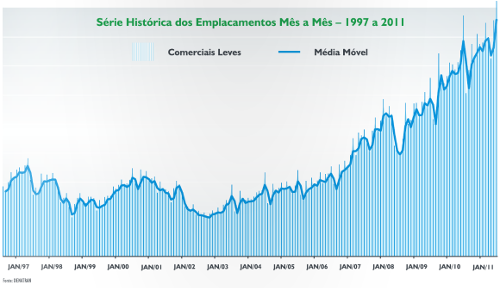
\includegraphics[scale=0.8]{imgs/emplacamentos.png}
%   \end{center}
%   \caption{Crescimento mensal no número de emplacamentos de veículos comerciais leves no período 1997 a 2011 \citep{fenabrave:2013:online}.} 
%   \label{fig:fenabreve}
% \end{figure}

A falta de planejamento urbano e o crescente aumento de veículos, a péssima qualidade do transporte público no Brasil e o excessivo número de acidentes de trânsito são umas das principais causas de congestionamentos. Nos últimos anos, milhões de pessoas perderam tempo e dinheiro devido a problemas relacionados ao trânsito \citep{pamela:2012:masther}. Diante desse fato, a administração pública deve priorizar o assunto mobilidade, como tem sido feito nas principais regiões metropolitanas brasileiras. Através de pesquisas pode-se levantar dados que contribuem para análise e simulação do tráfego. Informações como fluxo de veículos, volume de tráfego e matriz O/D (origem/destino) são de grande relevância no estudo dessa área, formando uma base teórica sólida para ser utilizada na resolução de problemas dessa natureza.

Na área de simulação do tráfego existem várias empresas atuantes: \cite{vissim:2013:online} é atualmente a líder mundial de mercado em simulação de fluxo de tráfego multi-modal de microregiões. Outras companhias, \cite{arcady:2013:online} e \cite{citilabs:2013:online}, também fornecem produtos com capacidades de predição, simulação de congestionamentos, atrasos, acidentes, além de gerar relatórios detalhados e animações 2D e 3D. SUMO - \textit{Simulation of Urban MObility} é uma alternativa \textit{open source}\footnote{O termo código aberto, ou \textit{open source} em inglês, foi criado pela OSI e refere-se a \textit{software} livre. Mais informações em \url{http://opensource.org}} e gratuita para simulação do tráfego, diferente dos produtos proprietários e de alto custo citados anteriormente \citep{SUMO2011}.

Segundo \cite{dnit:2011:online}, o PNCT - Plano Nacional de Contagem de Trânsito vem armazenando nos últimos anos importantes dados de volume de tráfego e já possui uma significativa série histórica desses dados. A informação coletada é de grande importância pois seus resultados são subsídios básicos para estudos econômicos, projetos rodoviários e planejamento de tráfego, além do papel essencial no estabelecimento de critérios para o cumprimento das seguintes finalidades:

\begin{itemize}
  \item Planejar o sistema rodoviário;
  \item Programar necessidades e prioridades de melhorias no sistema rodoviário;
  \item Estabelecer as tendências de tráfego no futuro;
  \item Avaliar o fluxo existente de tráfego em relação ao sistema rodoviário atual;
  \item Justificar e planejar o policiamento;
  \item Estudos de localização de postos de pesagem, socorro médico emergencial, etc.;
  \item Projetar pavimento, obras de arte, seção transversal e outros elementos de rodovia \citep{dnit:2011:online}. 
\end{itemize}

Existem métodos manuais e automáticos para realização das contagens volumétrica e classificatória, que normalmente são de alto custo financeiro. De acordo com a forma de instalação dos equipamentos de contagem, tais métodos podem ser invasivos ou não-invasivos. Os métodos invasivos necessitam de instalações junto ou sob a camada asfáltica. Já os métodos não-invasivos normalmente utilizam câmeras, sensores ou instalações sobre o solo \citep{goldner:2009:misc}.

Este trabalho tem como propósito desenvolver um método computacional de simples implementação, configuração, instalação e operação, capaz de realizar a contagem volumétrica de veículos de forma não-invasiva e que possa ser utilizado como uma alternativa de baixo custo financeiro, se comparado aos sitemas de contagem volumétrica convencionais.

\section{Objetivos} % (fold)
\label{sec:objetivos}

O objetivo principal do trabalho é desenvolver um sistema de visão computacional que auxilie na análise das condições do tráfego urbano. São os objetivos específicos deste estudo:
\begin{itemize}
  \item Entender a utilização de um sistema de visão para problemas de transporte;
  \item Realizar a contagem volumétrica dos veículos através de um método não-invasivo de simples implementação;
  \item Analisar as condições do tráfego urbano através de imagens coletadas por uma câmera digital;
  \item Através da análise dos resultados, determinar a qualidade do método e identificar pontos de acerto e erro que podem ser trabalhados.
\end{itemize}

% section objetivos (end)

% \section{Apresentação da Empresa} % (fold)
% \label{sec:apresenta_o_da_empresa}

% TODO: não é mais empresa

% A NunesCV é uma startup que foi criada no início de 2013 e desenvolve soluções e produtos de tecnologia para o setor de serviços. A empresa desenvolve sistemas baseados em visão computacional, como um produto para leitura automática de cartões de ponto utilizando tecnologia própria de Reconhecimento Ótico de Caracteres (OCR).

% Outro tipo de aplicação desenvolvida pela empresa é um sistema de gerenciamento remoto de uma rede de mídia indoor, que são televisões instaladas em pontos comerciais estratégicos anunciando informações úteis para os usuários. Cada ponto pode ter o conteúdo atualizado em tempo real via Internet, além de informar se a televisão está ligada e se o conteúdo está correto. A empresa desenvolve o software para um sistema embutido que controla o aparelho, o sistema web de gerenciamento e atualização de conteúdo e especifica o hardware necessário para o funcionamento do sistema.

% section apresenta_o_da_empresa (end)

\section{Organização do Texto} % (fold)
\label{sec:organiza_o_do_texto}

A monografia está dividida em seis capítulos:

\begin{itemize}
  \item Capítulo \ref{cha:introdu_o} é introdutório e são apresentados alguns pontos que motivam e justificam o desenvolvimento do projeto, além de uma listagem dos objetivos específicos que definem o escopo do mesmo.
  \item Capítulo \ref{cha:contagem_de_ve_culos_e_monitoramento_do_tr_fego} apresenta as tecnologias de contagem volumétrica e classificatória existentes. É também apresentado uma pesquisa bibliográfica sobre sistemas de visão computacional inseridos no contexto da Engenharia de Transporte.
  \item Capítulo \ref{cha:vis_o_computacional} introduz a teoria de visão computacional, contextualizando o leitor. Trata-se de uma apresentação da tecnologia com foco em conceitos e técnicas de processamento de imagens.
  \item Capítulo \ref{cha:metodologia} apresenta a metodologia para contagem volumétrica automática de veículos. As técnicas utilizadas, a sequência de operações, as imagens de processamento, as condições de captura, a estrutura do software e os métodos para análise de resultados são mostrados e explicados. 
  \item Capítulo \ref{cha:testes_e_resultados} apresenta os resultados e a validação das contagens; uma análise crítica do método proposto mostrando como as características da cena influenciam no resultado. 
  \item Capítulo \ref{cha:considera_es_finais} são feitas as conclusões e as considerações finais do trabalho, bem como recomendações para trabalhos futuros.
\end{itemize}


% section organiza_o_do_texto (end)